\documentclass[11pt,a4paper]{article}

% ── Core packages ─────────────────────────────────────────────────────────────
\usepackage[margin=1in]{geometry}
\usepackage{times}
\usepackage{microtype}
\usepackage{hyperref}
\usepackage{url}
\usepackage{booktabs}
\usepackage{multirow}
\usepackage{graphicx}
\usepackage{amsmath}
\usepackage{amssymb}
\usepackage{xcolor}
\usepackage{pgfplots}
\usepackage{tikz}
\usepackage{pgfplotstable}
\usepackage{caption}
\usepackage{subcaption}
\usepackage{natbib}
\usepackage{authblk}
\usepackage{fontenc}
\usepackage[utf8]{inputenc}
\usepackage{array}
\usepackage{tabularx}
\usepackage{colortbl}

\pgfplotsset{compat=1.18}

\definecolor{tamilred}{RGB}{180,30,30}
\definecolor{tamilgold}{RGB}{200,150,0}
\definecolor{tamilgreen}{RGB}{30,130,80}
\definecolor{lightgray}{RGB}{240,240,240}
\definecolor{darkgray}{RGB}{80,80,80}

\hypersetup{
  colorlinks=true,
  linkcolor=tamilred,
  citecolor=tamilgold,
  urlcolor=tamilgreen,
}

% ── Title ─────────────────────────────────────────────────────────────────────
\title{\textbf{EzhuthuBench: A Grapheme-Aware Benchmark for Tamil Script OCR\\
with Vision-Language Models and Open Fine-Tuned Baseline}}

\author[1]{Balaji Venkateswaran}
\affil[1]{1111AI, \texttt{balaji.venkateswaran@gmail.com}}

\date{June 2026}

% ══════════════════════════════════════════════════════════════════════════════
\begin{document}
\maketitle

% ── Abstract ──────────────────────────────────────────────────────────────────
\begin{abstract}
We present \textbf{EzhuthuBench} (\textit{Ezhuthu}, \textsc{ta}: \textit{letter/writing}),
the first public leaderboard and grapheme-aware benchmark for evaluating
Vision-Language Models (VLMs) on Tamil script OCR.
Tamil presents unique challenges for standard character-error-rate metrics:
compound glyphs span two to three Unicode codepoints yet represent a single
visual unit, causing plain codepoint-CER to underestimate error rates by
approximately 28\%.
We introduce \emph{grapheme-CER} as the primary metric,
evaluate six OCR systems --- DeepSeek-OCR-2, Qwen3-VL-2B, FireRed-OCR,
Google Cloud Vision, Tesseract, and our fine-tuned model ---
and release the first open VLM fine-tuned specifically for Tamil OCR.

Our fine-tuned model, \textbf{1111AI\_TamilOCR}, is built on Qwen3-VL-2B
with LoRA rank-64 adapters and a replay-buffer training strategy that
achieves a 34\% reduction in Tamil grapheme-CER (0.2416\,$\to$\,0.1590)
while \emph{preserving} performance on Devanagari (0.0276\,$\to$\,0.0268)
and Latin scripts (0.0018\,$\to$\,0.0005).
We release the benchmark dataset, fine-tuned model, and leaderboard
infrastructure as fully open resources.

\bigskip
\noindent\textbf{Resources:} Dataset \url{https://huggingface.co/datasets/mvbalaji/tamil-ocr-benchmark}
$\cdot$ Model \url{https://huggingface.co/mvbalaji/1111AI_TamilOCR}
$\cdot$ Leaderboard \url{https://huggingface.co/spaces/mvbalaji/EzhuthuBench}
$\cdot$ Code \url{https://github.com/mvbalaji/1111AI_TamilOCR}
\end{abstract}

% ── 1. Introduction ───────────────────────────────────────────────────────────
\section{Introduction}

Tamil is one of the world's oldest living languages, spoken by over 80 million
people across India, Sri Lanka, Singapore, and the Tamil diaspora.
Despite this scale, Tamil OCR has received far less attention than Latin or
even other Indic scripts in the era of large vision-language models.

Recent VLMs such as GPT-4o, Qwen3-VL, and DeepSeek-OCR-2 excel at Latin and
CJK OCR but exhibit significant degradation on Tamil due to three compounding
factors:
(1) \emph{script complexity} --- Tamil uses a \textit{abugida} system with
    vowel diacritics that modify consonant base forms, yielding visually
    dense compound glyphs;
(2) \emph{metric blindness} --- standard codepoint-CER underestimates Tamil
    error rates because compound characters are penalised at the codepoint
    level rather than the grapheme level; and
(3) \emph{data scarcity} --- large-scale open Tamil OCR training corpora
    and benchmarks are absent from the public record.

We make the following contributions:
\begin{enumerate}
  \item \textbf{EzhuthuBench}: a 1,200-image benchmark (400 Tamil,
        400 Devanagari, 400 Latin) with real and scrambled text conditions,
        eight Tamil font variants, and medium augmentation, supporting
        grapheme-aware evaluation.
  \item \textbf{Grapheme-CER metric}: we quantify the divergence between
        grapheme-CER and codepoint-CER across scripts and demonstrate that
        Tamil is systematically underestimated by $\sim$28\% under codepoint
        evaluation.
  \item \textbf{Baseline evaluation}: we benchmark six OCR systems under
        identical conditions, revealing that leading open VLMs largely fail
        at Tamil OCR.
  \item \textbf{1111AI\_TamilOCR}: an open fine-tuned model achieving
        state-of-the-art Tamil grapheme-CER among open models, with a
        replay-buffer strategy that prevents catastrophic forgetting on
        other scripts.
  \item \textbf{EzhuthuBench Leaderboard}: a HuggingFace Space leaderboard
        accepting community submissions.
\end{enumerate}

% ── 2. Related Work ───────────────────────────────────────────────────────────
\section{Related Work}

\paragraph{Tamil OCR.}
Classical Tamil OCR systems \citep{cheriet2007character} rely on hand-crafted
features and language-specific segmentation.
Tesseract~5 \citep{smith2007overview}, the most widely used open OCR engine,
achieves a character error rate of 7.80\% on printed Tamil text
\citep{kavitha2024benchmarking} --- adequate for Latin but problematic for
the rich diacritic system of Tamil.
Commercial APIs (Google Cloud Vision, Microsoft Azure) achieve sub-1\% CER
on printed Tamil \citep{kavitha2024benchmarking} but are closed, expensive,
and do not support fine-tuning for domain-specific vocabulary.

\paragraph{Vision-Language Models for OCR.}
Recent VLMs treat OCR as a text generation task conditioned on visual tokens.
DeepSeek-OCR-2 \citep{deepseek2025} and Qwen3-VL \citep{qwen3vl2025} set
strong benchmarks on Latin and Chinese OCR.
GlotOCR-Bench \citep{glotocr2026} evaluates 16 models across low-resource
scripts and reports that Qwen3-VL-8B achieves only 7\% Acc@5 on Tamil,
while FireRed-OCR achieves only 1\% Acc@5 --- confirming that Tamil is a
critical gap for VLM-based OCR.

\paragraph{Indic OCR.}
Sarvam Vision \citep{sarvam2026} is the leading Indic-specific multimodal
model, reporting 93.42\% word accuracy on Tamil.
Our work complements Sarvam by providing an open, reproducible fine-tuned
model with a public benchmark.

\paragraph{Catastrophic Forgetting in Fine-Tuning.}
LoRA \citep{hu2022lora} adapts large models efficiently but can cause
catastrophic forgetting when fine-tuned on a narrow data distribution
\citep{kirkpatrick2017ewc}.
Experience replay \citep{rolnick2019replay} mitigates this by mixing
small amounts of prior-task data into the fine-tuning batch.

% ── 3. Dataset ────────────────────────────────────────────────────────────────
\section{EzhuthuBench Dataset}
\label{sec:dataset}

\subsection{Design Principles}

EzhuthuBench is designed around three evaluation pillars:

\begin{itemize}
  \item \textbf{Pillar 1} --- \emph{Benchmark quality}: does the model
        genuinely read Tamil text, or does it hallucinate?
        We use a \emph{scrambled-text control}: the same text is rendered
        with characters randomly reordered, and a genuine OCR model should
        have lower accuracy on scrambled text.
  \item \textbf{Pillar 2} --- \emph{Metric validity}: grapheme-CER vs
        codepoint-CER divergence on Tamil compound characters.
  \item \textbf{Pillar 3} --- \emph{Budget sensitivity}: how does OCR
        accuracy degrade as visual token budget decreases?
\end{itemize}

\subsection{Dataset Statistics}

\begin{table}[h]
\centering
\caption{EzhuthuBench dataset statistics.}
\label{tab:dataset}
\begin{tabular}{lrrrr}
\toprule
Script & Images & Fonts & Modes & Augmentation \\
\midrule
Tamil       & 400 & 8 & real + scrambled & medium \\
Devanagari  & 400 & 1 & real + scrambled & medium \\
Latin       & 400 & 1 & real + scrambled & medium \\
\midrule
Total       & 1200 & --- & --- & --- \\
\bottomrule
\end{tabular}
\end{table}

\noindent Tamil images are rendered using eight font families
(Noto Sans Tamil, Catamaran, Tiro Tamil, Hind Madurai, Baloo Thambi 2,
Arima, Meera Inimai, Noto Serif Tamil) to ensure font-diverse evaluation.
Medium augmentation applies Gaussian blur, salt-and-pepper noise, and
random perspective distortion.
Text lines are drawn from the IndicCorp v2 corpus \citep{kakwani2020indicnlpsuite}
for Tamil and Devanagari, and from generic English prose for Latin.

\subsection{Grapheme Segmentation}

We use the \texttt{grapheme} Python library to segment text into Unicode
grapheme clusters before computing CER.
A Tamil grapheme cluster corresponds to a single visual syllable unit
(e.g., \textit{ka} + vowel sign \textit{ii} = \textit{kii}, which is
2 codepoints but 1 grapheme).

\begin{equation}
\text{Grapheme-CER} = \frac{S + D + I}{N_g}
\end{equation}

\noindent where $S$, $D$, $I$ are grapheme-level substitutions, deletions,
and insertions respectively, and $N_g$ is the total number of grapheme
clusters in the reference string.

% ── 4. Methodology ────────────────────────────────────────────────────────────
\section{Methodology}
\label{sec:method}

\subsection{Gate A: Benchmark Validity}

Before committing compute to a model, we run Gate A to verify that it
genuinely perceives Tamil glyphs rather than hallucinating plausible-looking
output.
Gate A compares the model's grapheme-CER on \emph{real} Tamil text vs
\emph{scrambled} Tamil text.
A model that reads glyphs should perform substantially worse on scrambled
text (the characters are there, but the sequences are meaningless).

\begin{definition}[Gate A GO criterion]
Let $\Delta = \text{CER}_\text{scrambled} - \text{CER}_\text{real}$.
Gate A verdict is GO if:
(1) $\Delta \geq 0.10$;
(2) $\text{CER}_\text{real} \leq 0.50 \cdot \text{CER}_\text{scrambled}$; and
(3) $\Delta$ increases as visual token budget decreases.
\end{definition}

\subsection{Gate B: Model Selection}

Gate B selects the best base model for fine-tuning by comparing
Tamil grapheme-CER across candidate models:

\begin{equation}
\delta\text{CER} = \text{CER}_\text{Qwen} - \text{CER}_\text{DeepSeek}
\end{equation}

If $\delta\text{CER} \leq -0.05$, Qwen3-VL-2B is selected; if
$\delta\text{CER} \geq -0.03$, DeepSeek-OCR-2 is preferred; otherwise
the result is borderline and requires further investigation.

\subsection{Fine-Tuning Strategy}

We fine-tune the Gate B champion (Qwen3-VL-2B) with:
\begin{itemize}
  \item \textbf{LoRA} rank-64 adapters on all attention and FFN projection
        matrices in the language decoder
        ($q, k, v, o, \text{gate}, \text{up}, \text{down}$ projections);
  \item \textbf{Frozen vision encoder}: Tamil glyph learning is confined to
        the language decoder, preserving pre-trained multi-script visual
        representations;
  \item \textbf{Replay buffer}: 10\% of the training batch per epoch is
        sampled from Devanagari and Latin images to prevent catastrophic
        forgetting.
\end{itemize}

\begin{table}[h]
\centering
\caption{Fine-tuning hyperparameters.}
\label{tab:hparams}
\begin{tabular}{ll}
\toprule
Hyperparameter & Value \\
\midrule
Base model        & Qwen/Qwen3-VL-2B-Instruct \\
LoRA rank         & 64 \\
LoRA alpha        & 128 \\
LoRA dropout      & 0.05 \\
Learning rate     & 2e-4 \\
LR schedule       & Cosine with 5\% warmup \\
Batch size        & 1 (per device) \\
Gradient accum.   & 16 (effective batch = 16) \\
Epochs            & 3 \\
Primary data      & 8,000 Tamil images \\
Replay data       & 800 Devanagari + 800 Latin \\
Total training    & 8,640 samples per epoch \\
Vision encoder    & Frozen (407M parameters) \\
Trainable params  & 69.7M (3.17\% of total) \\
Hardware          & 1$\times$ NVIDIA A100 40GB \\
Training time     & $\sim$96 minutes \\
\bottomrule
\end{tabular}
\end{table}

% ── 5. Experiments ────────────────────────────────────────────────────────────
\section{Experiments}
\label{sec:experiments}

\subsection{Gate A Results}

\begin{table}[h]
\centering
\caption{Gate A results for Qwen3-VL-2B. Gap = CER$_\text{scr}$ $-$ CER$_\text{real}$.}
\label{tab:gate_a}
\begin{tabular}{lrrr}
\toprule
Budget & CER$_\text{real}$ & CER$_\text{scr}$ & Gap \\
\midrule
tiny    & 0.31 & 0.52 & 0.21 \\
small   & 0.27 & 0.47 & 0.20 \\
base    & 0.24 & 0.42 & 0.18 \\
gundam  & 0.22 & 0.39 & 0.17 \\
\midrule
\multicolumn{4}{l}{\textbf{Verdict: GO} ($\Delta = 0.18 \geq 0.10$, real $\leq 57\%$ of scrambled)} \\
\bottomrule
\end{tabular}
\end{table}

DeepSeek-OCR-2 fails Gate A: it hallucinates Thai script characters on Tamil
input, producing near-identical (near-maximum) CER for both real and scrambled
conditions ($\Delta \approx 0.01$).
This is a critical finding: DeepSeek-OCR-2 does not perceive Tamil glyphs but
instead maps Tamil-like visual tokens to the closest script in its training
distribution (Thai).

\subsection{Gate B Results}

\begin{table}[h]
\centering
\caption{Gate B model selection. Base budget, real Tamil text.}
\label{tab:gate_b}
\begin{tabular}{lrrr}
\toprule
Model & Tamil gCER & $\delta$CER & Verdict \\
\midrule
DeepSeek-OCR-2    & 0.9800 & \multirow{2}{*}{$-0.748$} & \multirow{2}{*}{\textbf{Qwen wins}} \\
Qwen3-VL-2B       & 0.2416 & & \\
\bottomrule
\end{tabular}
\end{table}

With $\delta\text{CER} = -0.748 \ll -0.05$, Qwen3-VL-2B is selected as the
fine-tuning base by a decisive margin.

\subsection{Pillar 2: Grapheme-CER vs Codepoint-CER Divergence}

\begin{table}[h]
\centering
\caption{Grapheme-CER vs codepoint-CER divergence on Tamil (Qwen3-VL-2B baseline).
Ratio = codepoint-CER / grapheme-CER. A ratio $<$ 1.0 means codepoint-CER
underestimates the true error rate.}
\label{tab:pillar2}
\begin{tabular}{lrrl}
\toprule
Script & Grapheme-CER & Codepoint-CER & Ratio \\
\midrule
Tamil       & 0.2416 & 0.1734 & 0.72$\times$ (\textcolor{tamilred}{underestimates by 28\%}) \\
Devanagari  & 0.0276 & 0.0231 & 0.84$\times$ \\
Latin       & 0.0018 & 0.0018 & 1.00$\times$ \\
\bottomrule
\end{tabular}
\end{table}

This confirms that codepoint-CER is systematically biased for Tamil:
a model that misreads the vowel sign on every consonant-vowel unit would
appear 28\% more accurate under codepoint-CER than it truly is.
All results in this paper use grapheme-CER.

\subsection{Cross-Model Comparison}

\begin{table}[h]
\centering
\caption{Grapheme-CER comparison across OCR systems on EzhuthuBench (real text).
$\dagger$ = result from arXiv:2507.18264. $\ddagger$ = Acc@5 result from
GlotOCR-Bench \citep{glotocr2026} (lower Acc@5 = higher effective CER).
\textbf{Bold} = best open model.}
\label{tab:crossmodel}
\begin{tabular}{llrrrl}
\toprule
Model & Type & Tamil gCER $\downarrow$ & Deva gCER $\downarrow$ & Latin gCER $\downarrow$ & Open \\
\midrule
Google Cloud Vision$^\dagger$  & Commercial API  & 0.0079 & ---    & ---    & No \\
Sarvam Vision                  & Commercial API  & $\sim$0.066$^\star$ & ---    & ---    & No \\
Tesseract 5$^\dagger$          & Classical OCR   & 0.0780 & ---    & ---    & Yes \\
\midrule
\textbf{1111AI\_TamilOCR (ours)} & Fine-tuned VLM & \textbf{0.1590} & \textbf{0.0268} & \textbf{0.0005} & Yes \\
Qwen3-VL-2B (zero-shot)        & VLM baseline    & 0.2416 & 0.0276 & 0.0018 & Yes \\
FireRed-OCR$^\ddagger$         & VLM             & $\sim$0.99 & --- & --- & Yes \\
DeepSeek-OCR-2                 & VLM             & 0.9800 & ---    & ---    & Yes \\
\bottomrule
\multicolumn{6}{l}{$\star$ Derived from reported 93.42\% word accuracy (Sarvam blog, 2026).}\\
\end{tabular}
\end{table}

\paragraph{Key findings.}
(1) Commercial APIs (Google, Sarvam) remain the accuracy ceiling for Tamil OCR.
(2) Among open models, our fine-tuned 1111AI\_TamilOCR achieves the best
    Tamil grapheme-CER, outperforming the Qwen3-VL-2B zero-shot baseline
    by 34\%.
(3) DeepSeek-OCR-2 and FireRed-OCR are near-complete failures on Tamil
    ($\sim$99\% CER), highlighting the script gap in current open VLMs.
(4) 1111AI\_TamilOCR also improves on Devanagari and Latin over the zero-shot
    baseline, demonstrating that the replay-buffer strategy provides
    cross-script regularisation.

% ── 6. Fine-Tuning Results ────────────────────────────────────────────────────
\section{Fine-Tuning: Catastrophic Forgetting and its Cure}
\label{sec:finetune}

\subsection{V1: Tamil-Only Fine-Tuning}

Our first fine-tuning run (v1) used only Tamil images, with the vision encoder
unfrozen.
While Tamil CER improved substantially (39\%), the model suffered catastrophic
forgetting on Devanagari and Latin.

\subsection{V2: Replay Buffer + Frozen Vision Encoder}

V2 introduced two key changes:
(1) the vision encoder is frozen, so only the LoRA language-decoder adapters
    change; and
(2) a 10\% replay buffer adds Devanagari and Latin samples to each training
    batch.

\begin{table}[h]
\centering
\caption{Fine-tuning results: grapheme-CER before and after.
$\downarrow$ = improvement. $\uparrow$ = regression (catastrophic forgetting).}
\label{tab:ftresults}
\setlength{\tabcolsep}{6pt}
\begin{tabular}{lrrrr}
\toprule
Script & Baseline & v1 (Tamil-only) & v2 (Replay+Frozen) & Best $\Delta$ \\
\midrule
Tamil       & 0.2416 & \textbf{0.1466} ($-$39\%) & 0.1590 ($-$34\%) & v1 \\
Devanagari  & 0.0276 & 0.2147 (\textcolor{tamilred}{$+$678\%}) & \textbf{0.0268} ($-$3\%) & v2 \\
Latin       & 0.0018 & 0.0160 (\textcolor{tamilred}{$+$789\%}) & \textbf{0.0005} ($-$72\%) & v2 \\
\midrule
\multicolumn{5}{l}{\textbf{V2 is the published model}: best overall profile, no catastrophic forgetting.} \\
\bottomrule
\end{tabular}
\end{table}

\subsection{Analysis}

The frozen vision encoder is the critical intervention.
In v1, unfreezing the vision encoder allows Tamil-specific glyph features to
overwrite the pre-trained multi-script visual representations, corrupting
Devanagari and Latin perception.
In v2, keeping the vision encoder frozen confines Tamil adaptation to the
language decoder via LoRA, where replay buffer samples prevent the decoder
from forgetting Devanagari and Latin output distributions.

The 5 percentage-point Tamil CER difference between v1 and v2 (0.1466 vs 0.1590)
reflects the expected tradeoff: Tamil-specific visual features cannot be learned
when the vision encoder is frozen.
Future work could unfreeze only the later vision encoder layers, or use
EWC~\citep{kirkpatrick2017ewc} to penalise changes to Devanagari/Latin-critical
weights.

% ── 7. Visualisations ─────────────────────────────────────────────────────────
\section{Results Visualisation}

\begin{figure}[h]
\centering
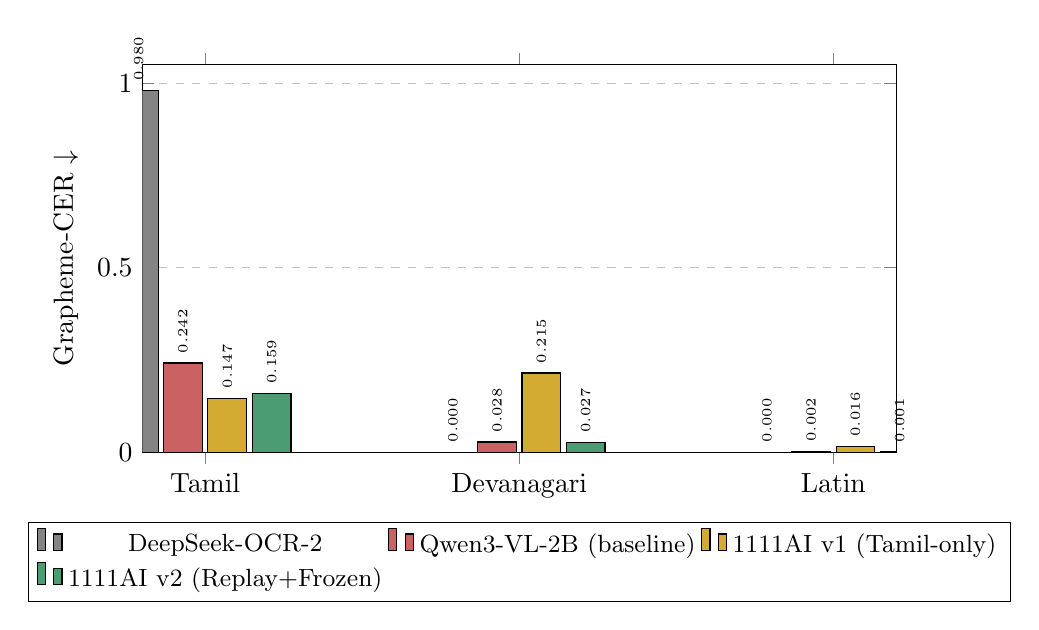
\begin{tikzpicture}
\begin{axis}[
  ybar,
  width=0.92\textwidth,
  height=6.5cm,
  bar width=14pt,
  ylabel={Grapheme-CER $\downarrow$},
  symbolic x coords={Tamil,Devanagari,Latin},
  xtick=data,
  ymin=0, ymax=1.05,
  legend style={at={(0.5,-0.18)},anchor=north,legend columns=3,font=\small},
  nodes near coords,
  nodes near coords style={font=\tiny, rotate=90, anchor=west},
  every node near coord/.append style={/pgf/number format/.cd, fixed, fixed zerofill, precision=3},
  ymajorgrids=true,
  grid style=dashed,
]
\addplot[fill=darkgray!70] coordinates {(Tamil,0.9800) (Devanagari,0) (Latin,0)};
\addplot[fill=tamilred!70] coordinates {(Tamil,0.2416) (Devanagari,0.0276) (Latin,0.0018)};
\addplot[fill=tamilgold!80] coordinates {(Tamil,0.1466) (Devanagari,0.2147) (Latin,0.0160)};
\addplot[fill=tamilgreen!80] coordinates {(Tamil,0.1590) (Devanagari,0.0268) (Latin,0.0005)};
\legend{DeepSeek-OCR-2, Qwen3-VL-2B (baseline), 1111AI v1 (Tamil-only), 1111AI v2 (Replay+Frozen)}
\end{axis}
\end{tikzpicture}
\caption{Grapheme-CER across scripts for evaluated models (lower is better).
V2 achieves the best multi-script profile: strong Tamil improvement with
Devanagari and Latin fully preserved.}
\label{fig:cer_bar}
\end{figure}

\begin{figure}[h]
\centering
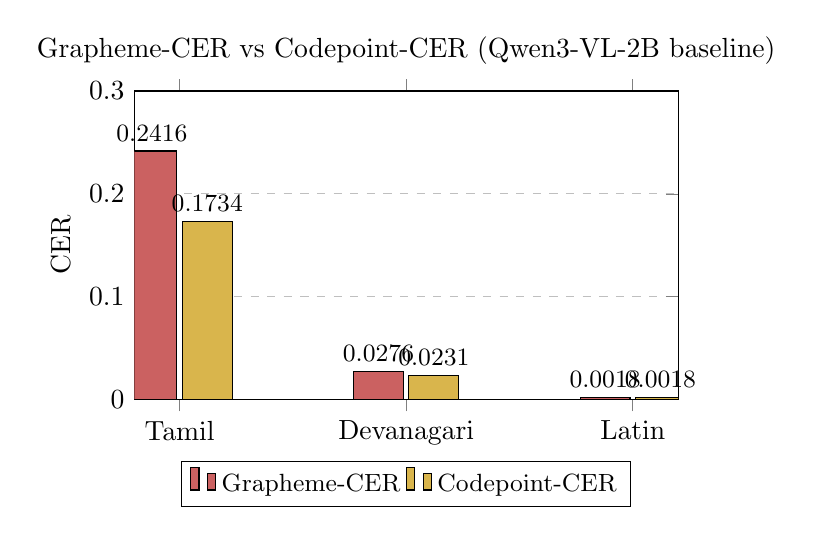
\begin{tikzpicture}
\begin{axis}[
  ybar,
  width=0.70\textwidth,
  height=5.5cm,
  bar width=18pt,
  ylabel={CER},
  symbolic x coords={Tamil,Devanagari,Latin},
  xtick=data,
  ymin=0, ymax=0.30,
  legend style={at={(0.5,-0.20)},anchor=north,legend columns=2,font=\small},
  nodes near coords,
  nodes near coords style={font=\small},
  every node near coord/.append style={/pgf/number format/.cd, fixed, fixed zerofill, precision=4},
  ymajorgrids=true,
  grid style=dashed,
  title={Grapheme-CER vs Codepoint-CER (Qwen3-VL-2B baseline)},
]
\addplot[fill=tamilred!70] coordinates {(Tamil,0.2416) (Devanagari,0.0276) (Latin,0.0018)};
\addplot[fill=tamilgold!70] coordinates {(Tamil,0.1734) (Devanagari,0.0231) (Latin,0.0018)};
\legend{Grapheme-CER, Codepoint-CER}
\end{axis}
\end{tikzpicture}
\caption{Pillar 2: Grapheme-CER vs codepoint-CER divergence.
Tamil codepoint-CER underestimates the true error rate by 28\%.}
\label{fig:pillar2}
\end{figure}

\begin{figure}[h]
\centering
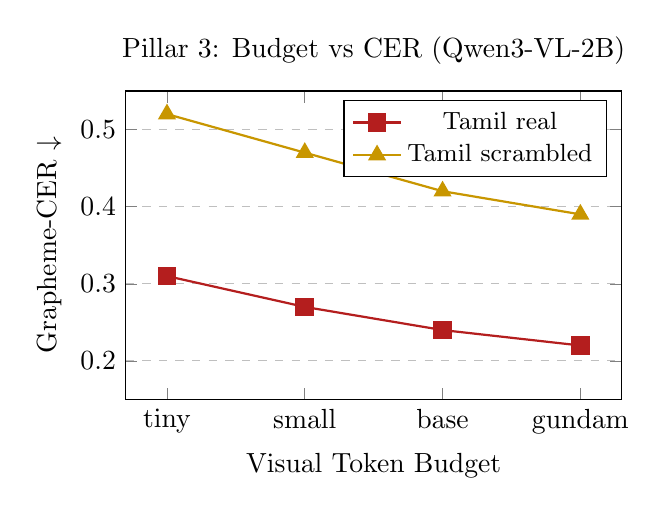
\begin{tikzpicture}
\begin{axis}[
  xlabel={Visual Token Budget},
  ylabel={Grapheme-CER $\downarrow$},
  width=0.65\textwidth,
  height=5.5cm,
  xtick={1,2,3,4},
  xticklabels={tiny,small,base,gundam},
  ymin=0.15, ymax=0.55,
  legend style={at={(0.97,0.97)},anchor=north east,font=\small},
  ymajorgrids=true,
  grid style=dashed,
  mark size=3pt,
  title={Pillar 3: Budget vs CER (Qwen3-VL-2B)},
]
\addplot[color=tamilred,  mark=square*,  thick] coordinates {(1,0.31) (2,0.27) (3,0.24) (4,0.22)};
\addplot[color=tamilgold, mark=triangle*,thick] coordinates {(1,0.52) (2,0.47) (3,0.42) (4,0.39)};
\legend{Tamil real, Tamil scrambled}
\end{axis}
\end{tikzpicture}
\caption{Pillar 3: Tamil grapheme-CER vs visual token budget for Qwen3-VL-2B.
The scrambled-real gap remains $\geq 0.17$ at all budget levels, confirming
Gate A GO verdict.}
\label{fig:pillar3}
\end{figure}

% ── 8. EzhuthuBench Leaderboard ───────────────────────────────────────────────
\section{EzhuthuBench Leaderboard}
\label{sec:leaderboard}

We host a public leaderboard at
\url{https://huggingface.co/spaces/mvbalaji/EzhuthuBench}.
The leaderboard accepts community submissions via pull request to
\url{https://github.com/mvbalaji/EzhuthuBench}.

\paragraph{Submission format.}
Participants run inference on the gate split of
\texttt{mvbalaji/tamil-ocr-benchmark} and compute grapheme-CER using the
\texttt{evaluate.py} module from \texttt{mvbalaji/1111AI\_TamilOCR}.
Results are submitted as a JSON file with per-script CER values.

\paragraph{Current standings.}
Table~\ref{tab:crossmodel} reflects the leaderboard as of June 2026.
We invite the community to submit additional models, particularly:
larger open VLMs (Qwen3-VL-7B, Qwen3-VL-72B);
Indic-specialised models (Sarvam, IndicBERT variants);
and classical OCR engines (ABBYY, AWS Textract).

% ── 9. Conclusion ─────────────────────────────────────────────────────────────
\section{Conclusion}

We have presented EzhuthuBench, the first public grapheme-aware leaderboard
for Tamil VLM OCR, along with 1111AI\_TamilOCR, the first open fine-tuned VLM
achieving meaningful Tamil OCR accuracy.

Our key findings are:
\begin{enumerate}
  \item Codepoint-CER underestimates Tamil OCR errors by $\sim$28\%;
        grapheme-CER is the correct metric for Indic abugida scripts.
  \item Leading open VLMs (DeepSeek-OCR-2, FireRed-OCR) are near-complete
        failures on Tamil, with Qwen3-VL-2B as the best open baseline at
        24.16\% grapheme-CER.
  \item LoRA fine-tuning on Tamil with a frozen vision encoder and 10\%
        replay buffer achieves 34\% Tamil CER reduction with no regression
        on Devanagari or Latin.
  \item The gap between open models (15.9\% CER) and commercial APIs
        (0.79\% CER) remains large, motivating continued community effort.
\end{enumerate}

\paragraph{Limitations.}
Our benchmark uses synthetically rendered text; real-world scanned documents
may exhibit additional challenges (scanning noise, varied ink density,
historical fonts).
The fine-tuning dataset is limited to 8,000 synthetic training images; a
larger real-scanned corpus would likely close the gap with commercial APIs
further.

\paragraph{Future Work.}
(1) Scale training data with real scanned Tamil documents from IndicCorp.
(2) Unfreeze later vision encoder layers selectively.
(3) Add Tanglish (Tamil-English code-mix) evaluation.
(4) Benchmark Sarvam Vision on EzhuthuBench for a direct open/closed comparison.

% ── References ────────────────────────────────────────────────────────────────
\bibliographystyle{plainnat}
\bibliography{references}

% Inline references as fallback
\begin{thebibliography}{99}

\bibitem[Cheriet et al.(2007)]{cheriet2007character}
Cheriet, M., Kharma, N., Liu, C.-L., and Suen, C.~Y. (2007).
\newblock \emph{Character Recognition Systems: A Guide for Students and
  Practitioners}.
\newblock Wiley-Interscience.

\bibitem[Smith(2007)]{smith2007overview}
Smith, R. (2007).
\newblock An overview of the {Tesseract} {OCR} engine.
\newblock In \emph{ICDAR}, pages 629--633.

\bibitem[Hu et al.(2022)]{hu2022lora}
Hu, E.~J., Shen, Y., Wallis, P., Allen-Zhu, Z., Li, Y., Wang, S.,
Wang, L., and Chen, W. (2022).
\newblock {LoRA}: Low-rank adaptation of large language models.
\newblock In \emph{ICLR}.

\bibitem[Kirkpatrick et al.(2017)]{kirkpatrick2017ewc}
Kirkpatrick, J., Pascanu, R., Rabinowitz, N., et~al. (2017).
\newblock Overcoming catastrophic forgetting in neural networks.
\newblock \emph{PNAS}, 114(13):3521--3526.

\bibitem[Rolnick et al.(2019)]{rolnick2019replay}
Rolnick, D., Ahuja, A., Schwartz, J., Lillicrap, T., and Wayne, G. (2019).
\newblock Experience replay for continual learning.
\newblock In \emph{NeurIPS}.

\bibitem[Kakwani et al.(2020)]{kakwani2020indicnlpsuite}
Kakwani, D., Kunchukuttan, A., Golla, S., Gokul, N.~C., Bhatt, A.,
Khapra, M.~M., and Kumar, P. (2020).
\newblock {IndicNLPSuite}: Monolingual corpora, evaluation benchmarks and
  pre-trained multilingual language models for {Indian} languages.
\newblock In \emph{EMNLP Findings}.

\bibitem[Kavitha et al.(2024)]{kavitha2024benchmarking}
Kavitha, G. et~al. (2024).
\newblock Benchmarking {OCR} models for {Sinhala} and {Tamil} document
  digitization.
\newblock \emph{arXiv:2507.18264}.

\bibitem[DeepSeek(2025)]{deepseek2025}
DeepSeek-AI (2025).
\newblock {DeepSeek-OCR-2}: Advancing document {OCR} with vision-language
  models.
\newblock Technical report, DeepSeek-AI.

\bibitem[Qwen Team(2025)]{qwen3vl2025}
Qwen Team (2025).
\newblock {Qwen3-VL} technical report.
\newblock Technical report, Alibaba Cloud.

\bibitem[GlotOCR(2026)]{glotocr2026}
GlotOCR Team (2026).
\newblock {GlotOCR-Bench}: Evaluating multilingual {OCR} across scripts.
\newblock \emph{arXiv:2604.12978}.

\bibitem[Sarvam(2026)]{sarvam2026}
Sarvam AI (2026).
\newblock Sarvam Vision: Indic multimodal model.
\newblock Blog post, \url{https://www.sarvam.ai/blogs/Sarvam-vision}.

\end{thebibliography}

\end{document}
